En esta secci\'on revisaremos una familia de ecuaciones con coeficientes variables que tiene la particularidad de ser una de las pocas para las cuales se puede dar una descripci\'on completa de sus soluciones. Ya nos hemos encontrado con ella en la secci\'on de reducci\'on de orden: las ecuaciones $x^2y''-3xy'+4y=0$ y $x^2y''+3xy'+y=4\ln(x)$ pertenecen a esta familia. Veremos que, en el fondo, estas ecuaciones son ecuaciones de coeficientes constantes ``disfrazadas''.

\begin{definition}[Ecuaci\'on de Cauchy-Euler]
    Una ecuaci\'on del tipo
    \[
    x^n\dfrac{d^ny}{dx^n}+a_1x^{n-1}\dfrac{d^{n-1}y}{dx^{n-1}}+\cdots+a_{n-1}x\dfrac{dy}{dx}+a_ny=0,
    \]
    donde $a_i\in \mathbb{R}$, la llamaremos una \textbf{ecuaci\'on de Cauchy-Euler}. Trabajaremos en el intervalo $x>0$.
\end{definition}

Notemos que en $x=0$ el coeficiente de la derivada de mayor orden se anula, por lo que la ecuaci\'on es \emph{singular} en ese punto: all\'i no podemos aplicar el teorema de existencia y unicidad, y veremos que algunas soluciones no est\'an definidas o no son acotadas cerca de $x=0$. Por eso buscaremos soluciones en $x>0$ (el caso $x<0$ lo comentamos al final de la secci\'on).

\begin{remark}[La ecuaci\'on indicial]
    En particular, para el caso $n=2$ se tiene una ecuaci\'on del tipo:
    \[
    x^2y''+a_1xy'+a_2y=0.
    \]
    La forma de la ecuaci\'on sugiere buscar soluciones del tipo $y=x^r$: cada derivada baja la potencia en uno, y cada factor $x$ la sube en uno, de modo que todos los t\'erminos quedan con la misma potencia $x^r$. En efecto,
    \[
    y'=rx^{r-1},\qquad y''=r(r-1)x^{r-2},
    \]
    y al reemplazar obtenemos
    \[
    x^r\big[r(r-1)+a_1r+a_2\big]=0.
    \]
    Como $x^r\neq0$ para $x>0$, esto ocurre si y solo si
    \[
    r^2+(a_1-1)r+a_2=0.
    \]
    A esta ecuaci\'on la llamaremos la \textbf{ecuaci\'on indicial} de la ecuaci\'on de Cauchy-Euler. Notemos que \emph{no} es la que se obtendr\'ia ``copiando'' los coeficientes: el t\'ermino $r(r-1)$ hace que el coeficiente de $r$ sea $a_1-1$.
\end{remark}

La ecuaci\'on indicial, al igual que la ecuaci\'on auxiliar en coeficientes constantes, nos entrega tres casos para analizar.

\begin{theorem}
    Sea $x>0$ y sean $r_1,r_2$ las ra\'ices de la ecuaci\'on indicial $r^2+(a_1-1)r+a_2=0$. La soluci\'on general de $x^2y''+a_1xy'+a_2y=0$ es:
    \begin{enumerate}[label=\roman*)]
        \item Si $r_1\neq r_2$ son reales:
        \[
        y(x)=C_1x^{r_1}+C_2x^{r_2}.
        \]
        \item Si $r_1=r_2=r$ (ra\'iz doble, $r=\frac{1-a_1}{2}$):
        \[
        y(x)=C_1x^{r}+C_2x^{r}\ln(x).
        \]
        \item Si $r=\alpha\pm i\beta$ son complejas, con $\beta\neq0$:
        \[
        y(x)=C_1x^{\alpha}\cos\big(\beta\ln(x)\big)+C_2x^{\alpha}\sin\big(\beta\ln(x)\big).
        \]
    \end{enumerate}
\end{theorem}

\begin{proof}[Justificaci\'on]
    El caso i) es inmediato: $x^{r_1}$ y $x^{r_2}$ son soluciones, y son L.I. porque su cociente $x^{r_1-r_2}$ no es constante.

    En el caso ii), $y_1=x^r$ es soluci\'on y usamos reducci\'on de orden. En forma est\'andar $P(x)=\dfrac{a_1}{x}$, luego $e^{-\int P\,dx}=x^{-a_1}$. Como $2r=1-a_1$,
    \[
    y_2=x^r\int\dfrac{x^{-a_1}}{x^{2r}}\,dx=x^r\int\dfrac{x^{-a_1}}{x^{1-a_1}}\,dx=x^r\int\dfrac{dx}{x}=x^r\ln(x).
    \]

    En el caso iii), $x^{\alpha+i\beta}$ es una soluci\'on compleja. Escribiendo $x=e^{\ln(x)}$ y usando la f\'ormula de Euler,
    \[
    x^{\alpha+i\beta}=e^{(\alpha+i\beta)\ln(x)}=x^{\alpha}\Big[\cos\big(\beta\ln(x)\big)+i\sin\big(\beta\ln(x)\big)\Big].
    \]
    Como los coeficientes de la ecuaci\'on son reales, la parte real y la parte imaginaria son soluciones reales por separado, igual que en el caso de coeficientes constantes.
\end{proof}

\begin{figure}[h!]
    \centering
    \begin{subfigure}[b]{0.32\textwidth}
        \centering
        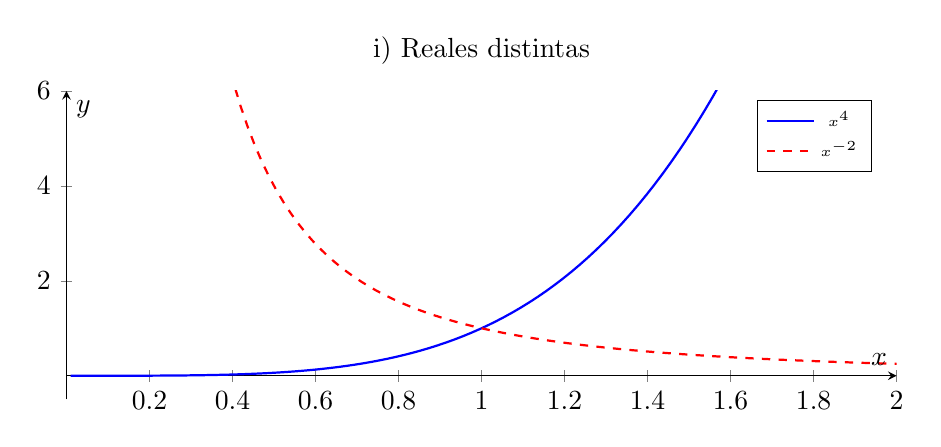
\begin{tikzpicture}
            \begin{axis}[
                axis lines = middle,
                xlabel = $x$, ylabel = {$y$},
                xmin=0, xmax=2, ymin=-0.5, ymax=6,
                restrict y to domain=-1:7,
                title = {i) Reales distintas},
                width=\textwidth, height=5.5cm,
                legend pos = north east,
                legend style={font=\tiny}
            ]
            \addplot[domain=0.01:2, samples=100, blue, thick] {x^4};
            \addlegendentry{$x^4$}
            \addplot[domain=0.3:2, samples=100, red, thick, dashed] {x^(-2)};
            \addlegendentry{$x^{-2}$}
            \end{axis}
        \end{tikzpicture}
    \end{subfigure}
    \hfill
    \begin{subfigure}[b]{0.32\textwidth}
        \centering
        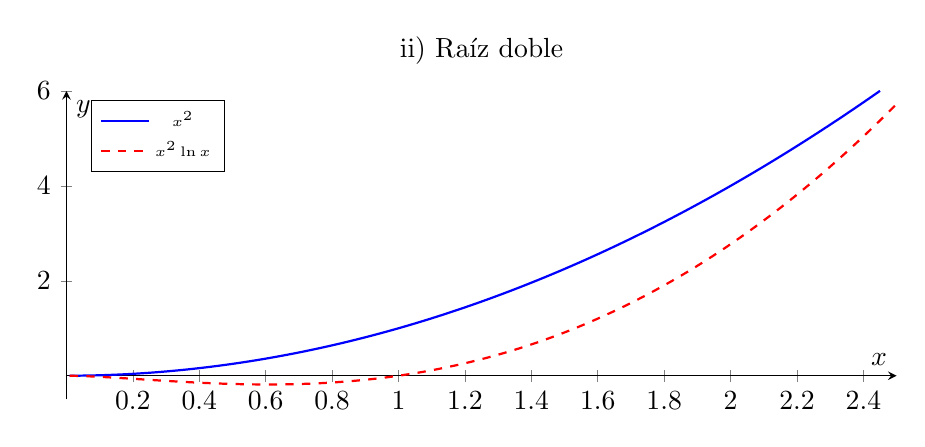
\begin{tikzpicture}
            \begin{axis}[
                axis lines = middle,
                xlabel = $x$, ylabel = {$y$},
                xmin=0, xmax=2.5, ymin=-0.5, ymax=6,
                title = {ii) Ra\'iz doble},
                width=\textwidth, height=5.5cm,
                legend pos = north west,
                legend style={font=\tiny}
            ]
            \addplot[domain=0.01:2.45, samples=100, blue, thick] {x^2};
            \addlegendentry{$x^2$}
            \addplot[domain=0.01:2.5, samples=100, red, thick, dashed] {x^2*ln(x)};
            \addlegendentry{$x^2\ln x$}
            \end{axis}
        \end{tikzpicture}
    \end{subfigure}
    \hfill
    \begin{subfigure}[b]{0.32\textwidth}
        \centering
        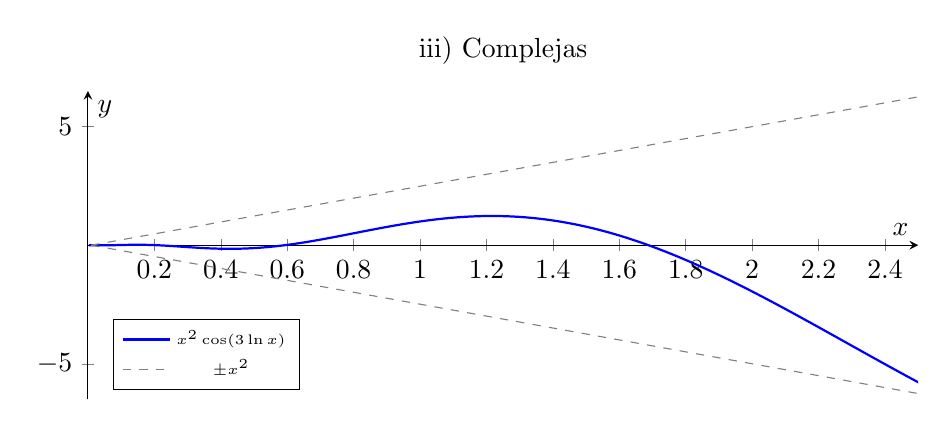
\begin{tikzpicture}
            \begin{axis}[
                axis lines = middle,
                xlabel = $x$, ylabel = {$y$},
                xmin=0, xmax=2.5, ymin=-6.5, ymax=6.5,
                title = {iii) Complejas},
                width=\textwidth, height=5.5cm,
                legend pos = south west,
                legend style={font=\tiny}
            ]
            \addplot[domain=-6:0.92, samples=400, blue, thick] ({exp(x)},{exp(2*x)*cos(deg(3*x))});
            \addlegendentry{$x^2\cos(3\ln x)$}
            \addplot[domain=0.01:2.5, samples=2, gray, dashed] {x^2};
            \addplot[domain=0.01:2.5, samples=2, gray, dashed, forget plot] {-x^2};
            \addlegendentry{$\pm x^2$}
            \end{axis}
        \end{tikzpicture}
    \end{subfigure}
    \caption{Soluciones t\'ipicas de cada caso. En i), $x^{-2}$ no est\'a acotada cerca de $x=0$; en ii), el factor $\ln(x)$ hace que $x^2\ln(x)$ sea negativa en $0<x<1$; en iii), la soluci\'on oscila entre las envolventes $\pm x^2$. En los tres casos se aprecia que $x=0$ es un punto especial.}
    \label{fig:euler_tres_casos}
\end{figure}

\subsection*{El cambio de variable $x=e^z$}

\begin{remark}[Cauchy-Euler como coeficientes constantes]
    Los tres casos del teorema se parecen demasiado a los de coeficientes constantes como para ser una coincidencia. La explicaci\'on es el cambio de variable
    \[
    x=e^z,\qquad\text{es decir,}\qquad z=\ln(x).
    \]
    Usando la regla de la cadena (ver el Ejercicio al final de la secci\'on), se obtiene
    \[
    x\dfrac{dy}{dx}=\dfrac{dy}{dz},\qquad x^2\dfrac{d^2y}{dx^2}=\dfrac{d^2y}{dz^2}-\dfrac{dy}{dz},
    \]
    con lo cual la ecuaci\'on $x^2y''+a_1xy'+a_2y=0$ se transforma en
    \[
    \dfrac{d^2y}{dz^2}+(a_1-1)\dfrac{dy}{dz}+a_2y=0,
    \]
    \textbf{una ecuaci\'on de coeficientes constantes}, cuya ecuaci\'on auxiliar es exactamente la ecuaci\'on indicial. Resolvi\'endola en $z$ y volviendo a $x$ mediante $z=\ln(x)$ obtenemos el siguiente diccionario:
    \begin{center}
    \renewcommand{\arraystretch}{1.5}
    \begin{tabular}{|c|c|}
    \hline
    \textbf{Coeficientes constantes (en $z$)} & \textbf{Cauchy-Euler (en $x=e^z$)} \\ \hline
    $e^{rz}$ & $x^{r}$ \\ \hline
    $z\,e^{rz}$ & $x^{r}\ln(x)$ \\ \hline
    $e^{\alpha z}\cos(\beta z)$,\ \ $e^{\alpha z}\sin(\beta z)$ & $x^{\alpha}\cos\big(\beta\ln(x)\big)$,\ \ $x^{\alpha}\sin\big(\beta\ln(x)\big)$ \\ \hline
    \end{tabular}
    \end{center}
\end{remark}

\begin{figure}[h!]
    \centering
    \begin{tikzpicture}[
        caja/.style={draw=bbe, fill=bbe!8, rounded corners=3pt, text width=5.6cm, align=center, minimum height=1.8cm, font=\small, text=black},
        flecha/.style={->, thick, draw=bbe},
        etiqueta/.style={font=\small, text=bbe, fill=white, inner sep=2pt}
    ]
        \node[caja] (A) at (0,0) {\textbf{Cauchy-Euler en $x$}\\[3pt] $x^2y''+a_1xy'+a_2y=0$};
        \node[caja] (B) at (8.2,0) {\textbf{Coeficientes constantes en $z$}\\[3pt] $\ddot y+(a_1-1)\dot y+a_2y=0$};
        \node[caja] (C) at (8.2,-3.2) {\textbf{Soluciones en $z$}\\[3pt] $e^{rz},\ ze^{rz},\ e^{\alpha z}\cos(\beta z),\ \ldots$};
        \node[caja] (D) at (0,-3.2) {\textbf{Soluciones en $x$}\\[3pt] $x^{r},\ x^{r}\ln x,\ x^{\alpha}\cos(\beta\ln x),\ \ldots$};
        \draw[flecha] (A) -- node[etiqueta, above] {$x=e^z$} (B);
        \draw[flecha] (B) -- node[etiqueta, right] {resolver} (C);
        \draw[flecha] (C) -- node[etiqueta, below] {$z=\ln(x)$} (D);
        \draw[flecha, dashed] (A) -- node[etiqueta, left] {probar $x^r$} (D);
    \end{tikzpicture}
    \caption{Dos caminos para resolver una ecuaci\'on de Cauchy-Euler: probar directamente $y=x^r$ (flecha discontinua), o transformarla en una ecuaci\'on de coeficientes constantes mediante $x=e^z$. Aqu\'i $\dot y$ denota la derivada respecto de $z$.}
    \label{fig:euler_cambio_variable}
\end{figure}

El cambio de variable tambi\'en explica una caracter\'istica curiosa de las soluciones del caso iii). Como la oscilaci\'on ocurre en la variable $z=\ln(x)$, sus ceros est\'an igualmente espaciados en $\ln(x)$, no en $x$: las oscilaciones se \emph{amontonan} cerca de $x=0$ y se \emph{estiran} cuando $x$ crece. La Figura~\ref{fig:euler_log} lo muestra para la ecuaci\'on $x^2y''+xy'+9y=0$, cuya ecuaci\'on indicial $r^2+9=0$ tiene ra\'ices $\pm3i$ y una de cuyas soluciones es $y=\cos(3\ln x)$.

\begin{figure}[h!]
    \centering
    \begin{subfigure}[b]{0.48\textwidth}
        \centering
        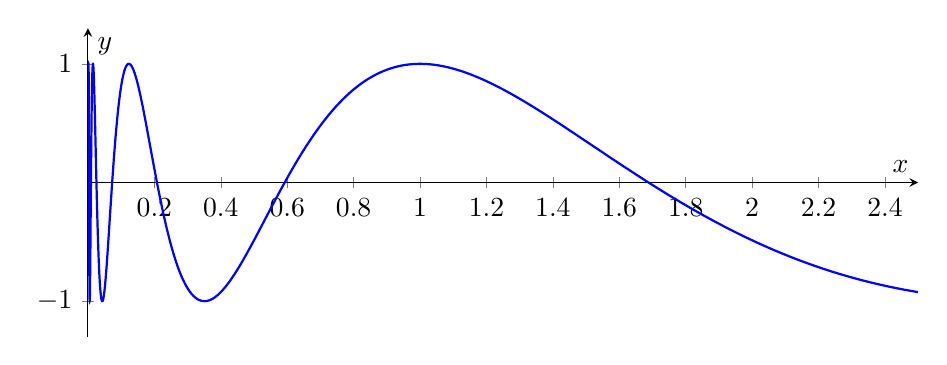
\begin{tikzpicture}
            \begin{axis}[
                axis lines = middle,
                xlabel = $x$, ylabel = {$y$},
                xmin=0, xmax=2.5, ymin=-1.3, ymax=1.3,
                width=\textwidth, height=5.5cm
            ]
            \addplot[domain=-7:0.916, samples=800, blue, thick] ({exp(x)},{cos(deg(3*x))});
            \end{axis}
        \end{tikzpicture}
        \caption{Eje $x$ en escala usual.}
    \end{subfigure}
    \hfill
    \begin{subfigure}[b]{0.48\textwidth}
        \centering
        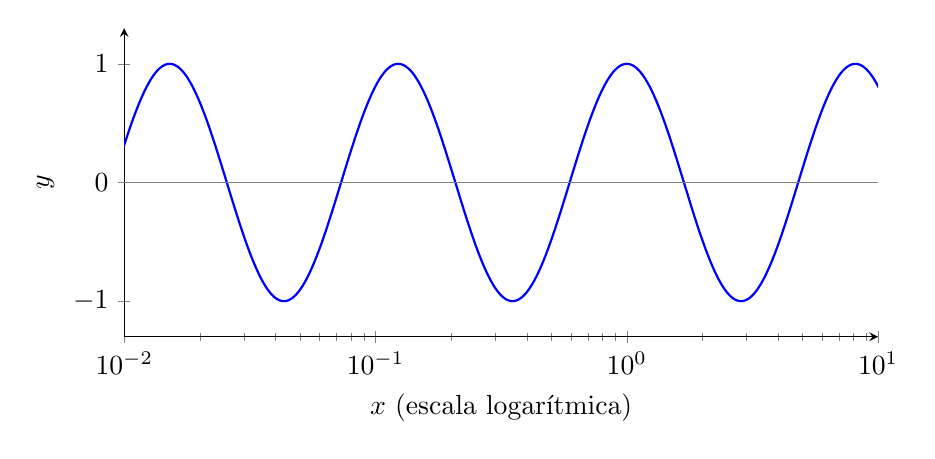
\begin{tikzpicture}
            \begin{axis}[
                xmode=log,
                axis lines = left,
                xlabel = {$x$ (escala logar\'itmica)}, ylabel = {$y$},
                xmin=0.01, xmax=10, ymin=-1.3, ymax=1.3,
                width=0.92\textwidth, height=5.5cm
            ]
            \addplot[domain=-4.61:2.31, samples=400, blue, thick] ({exp(x)},{cos(deg(3*x))});
            \addplot[domain=0.01:10, samples=2, gray, forget plot] {0};
            \end{axis}
        \end{tikzpicture}
        \caption{Eje $x$ en escala logar\'itmica.}
    \end{subfigure}
    \caption{La soluci\'on $y=\cos(3\ln x)$ de $x^2y''+xy'+9y=0$. En la escala usual, las oscilaciones se acumulan cerca de $x=0$ (infinitas oscilaciones en $0<x<1$). En escala logar\'itmica, es decir, en la variable $z=\ln(x)$, se ve una oscilaci\'on perfectamente regular: la de $\cos(3z)$.}
    \label{fig:euler_log}
\end{figure}

\subsection*{Ejemplos}

\begin{example}
    Considere la ecuaci\'on
    \[
    x^2y''-xy'-8y=0,\qquad x>0.
    \]
    Aqu\'i $a_1=-1$ y $a_2=-8$, por lo que la ecuaci\'on indicial es
    \[
    r^2+(-1-1)r-8=r^2-2r-8=(r-4)(r+2)=0,
    \]
    con ra\'ices reales y distintas $r_1=4$, $r_2=-2$. Con lo cual, la soluci\'on general es:
    \[
    y(x)=C_1x^4+C_2x^{-2}.
    \]
\end{example}

\begin{example}
    Resolvamos el problema de valor inicial
    \[
    x^2y''-3xy'+13y=0,\qquad y(1)=2,\qquad y'(1)=-5.
    \]
    En este caso $a_1=-3$, $a_2=13$, y la ecuaci\'on indicial es
    \[
    r^2-4r+13=0\Longrightarrow r=2\pm 3i,
    \]
    es decir, $\alpha=2$, $\beta=3$. Por lo tanto, la soluci\'on general es
    \[
    y(x)=x^2\Big[C_1\cos\big(3\ln(x)\big)+C_2\sin\big(3\ln(x)\big)\Big].
    \]
    Para imponer las condiciones iniciales necesitamos $y'$. Recordando que $\dfrac{d}{dx}\cos\big(3\ln(x)\big)=-\dfrac{3}{x}\sin\big(3\ln(x)\big)$ (regla de la cadena), obtenemos
    \[
    y'(x)=x\Big[(2C_1+3C_2)\cos\big(3\ln(x)\big)+(2C_2-3C_1)\sin\big(3\ln(x)\big)\Big].
    \]
    Como $\ln(1)=0$, al evaluar en $x=1$ los senos se anulan y los cosenos valen $1$:
    \[
    y(1)=C_1=2,\qquad y'(1)=2C_1+3C_2=-5,
    \]
    de donde $C_1=2$, $C_2=-3$. La soluci\'on buscada es:
    \[
    y(x)=2x^2\cos\big(3\ln(x)\big)-3x^2\sin\big(3\ln(x)\big).
    \]
\end{example}

\begin{figure}[h!]
    \centering
    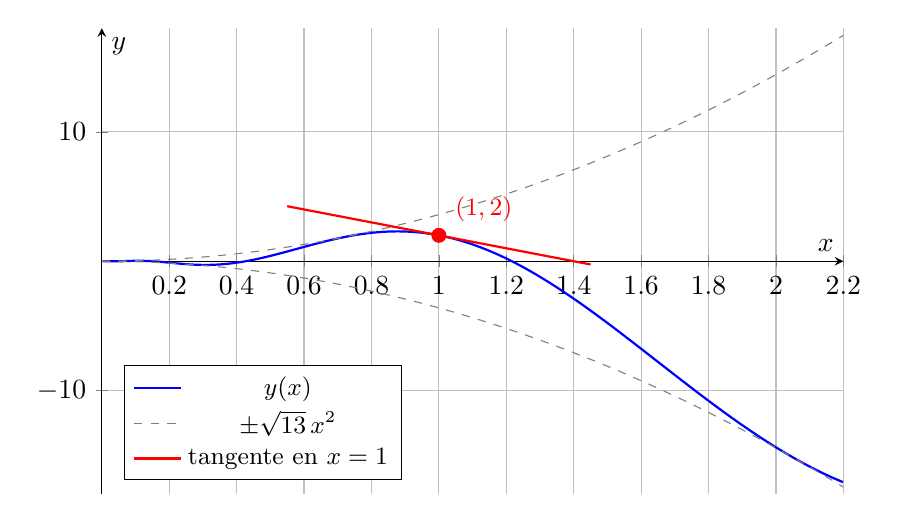
\begin{tikzpicture}
        \begin{axis}[
            axis lines = middle,
            xlabel = $x$, ylabel = {$y$},
            xmin=0, xmax=2.2, ymin=-18, ymax=18,
            grid = both,
            width = 11cm, height = 7.5cm,
            legend pos = south west,
            legend style={font=\small}
        ]
        \addplot[domain=-6:0.788, samples=500, blue, thick]
            ({exp(x)},{exp(2*x)*(2*cos(deg(3*x)) - 3*sin(deg(3*x)))});
        \addlegendentry{$y(x)$}
        \addplot[domain=0:2.2, samples=100, gray, dashed] {sqrt(13)*x^2};
        \addlegendentry{$\pm\sqrt{13}\,x^2$}
        \addplot[domain=0:2.2, samples=100, gray, dashed, forget plot] {-sqrt(13)*x^2};
        \addplot[domain=0.55:1.45, samples=2, red, thick] {2 - 5*(x-1)};
        \addlegendentry{tangente en $x=1$}
        \addplot[only marks, mark=*, mark size=2.5pt, red] coordinates {(1,2)};
        \node[red, anchor=south west, font=\small] at (axis cs:1.02,2.3) {$(1,2)$};
        \end{axis}
    \end{tikzpicture}
    \caption{Soluci\'on del PVI $x^2y''-3xy'+13y=0$, $y(1)=2$, $y'(1)=-5$. La curva pasa por el punto $(1,2)$ con pendiente $-5$ (recta roja), y oscila entre las envolventes $\pm\sqrt{13}\,x^2$ (la amplitud es $\sqrt{C_1^2+C_2^2}=\sqrt{13}$).}
    \label{fig:euler_pvi}
\end{figure}

\begin{example}
    Consideremos la ecuaci\'on no homog\'enea
    \[
    x^2y''-3xy'+4y=x^2\ln(x),\qquad x>0.
    \]
    La ecuaci\'on indicial es
    \[
    r^2-4r+4=(r-2)^2=0\Longrightarrow r_1=r_2=2,
    \]
    por lo que la soluci\'on de la ecuaci\'on homog\'enea es
    \[
    y_h(x)=C_1x^2+C_2x^2\ln(x),
    \]
    tal como obtuvimos por reducci\'on de orden en la secci\'on anterior. Para encontrar una soluci\'on particular usamos variaci\'on de par\'ametros. Primero llevamos la ecuaci\'on a forma est\'andar dividiendo por $x^2$:
    \[
    y''-\dfrac{3}{x}y'+\dfrac{4}{x^2}y=\ln(x),
    \]
    de modo que $F(x)=\ln(x)$. Con $y_1=x^2$, $y_2=x^2\ln(x)$, el Wronskiano es (como ya vimos con la f\'ormula de Abel) $W[y_1,y_2]=x^3$. Entonces
    \[
    u'=-\dfrac{y_2F}{W}=-\dfrac{x^2\ln(x)\cdot\ln(x)}{x^3}=-\dfrac{(\ln x)^2}{x},\qquad v'=\dfrac{y_1F}{W}=\dfrac{x^2\ln(x)}{x^3}=\dfrac{\ln(x)}{x}.
    \]
    Ambas integrales se resuelven con la sustituci\'on $s=\ln(x)$, $ds=\dfrac{dx}{x}$:
    \[
    u=-\dfrac{(\ln x)^3}{3},\qquad v=\dfrac{(\ln x)^2}{2}.
    \]
    Luego,
    \[
    y_p=u\,y_1+v\,y_2=-\dfrac{(\ln x)^3}{3}\,x^2+\dfrac{(\ln x)^2}{2}\,x^2\ln(x)=\dfrac{x^2(\ln x)^3}{6},
    \]
    y la soluci\'on general es
    \[
    y(x)=C_1x^2+C_2x^2\ln(x)+\dfrac{x^2(\ln x)^3}{6}.
    \]
\end{example}

\begin{remark}[El caso $x<0$]
    Si necesitamos soluciones en $x<0$, basta reemplazar $x$ por $|x|$ en las f\'ormulas del teorema; por ejemplo, en el caso de ra\'ices reales distintas, $y=C_1|x|^{r_1}+C_2|x|^{r_2}$. Esto se puede comprobar con el cambio de variable $x=-t$, que transforma la ecuaci\'on en otra ecuaci\'on de Cauchy-Euler en $t>0$ con los mismos coeficientes.
\end{remark}

\begin{exercise}
    Considere la ecuaci\'on
    \[
    x^2y''+a_1xy'+a_2y=0,\qquad x>0.
    \]
    \begin{enumerate}[label=\alph*)]
        \item Pruebe que el cambio de variable $x=e^z$ satisface
        \[
        x\dfrac{dy}{dx}=\dfrac{dy}{dz},\qquad x^2\dfrac{d^2y}{dx^2}=\dfrac{d^2y}{dz^2}-\dfrac{dy}{dz}.
        \]
        \textit{Indicaci\'on:} use que $\dfrac{dz}{dx}=\dfrac{1}{x}$ y la regla de la cadena.
        \item Concluya que la ecuaci\'on se transforma en
        \[
        \dfrac{d^2y}{dz^2}+(a_1-1)\dfrac{dy}{dz}+a_2y=0.
        \]
        \item Pruebe que si $y_1(z),y_2(z)$ son soluciones de esta \'ultima ecuaci\'on, entonces $y_1\big(\ln(x)\big)$ e $y_2\big(\ln(x)\big)$ son soluciones de la ecuaci\'on original.
    \end{enumerate}
\end{exercise}

\begin{exercise}
    La definici\'on de ecuaci\'on de Cauchy-Euler es v\'alida para cualquier orden $n$, y la idea de probar $y=x^r$ sigue funcionando. Considere la ecuaci\'on de tercer orden
    \[
    x^3y'''+xy'-y=0,\qquad x>0.
    \]
    \begin{enumerate}[label=\alph*)]
        \item Pruebe que al reemplazar $y=x^r$ se obtiene la ecuaci\'on indicial $(r-1)^3=0$.
        \item Por analog\'ia con el caso de una ra\'iz doble, proponga tres soluciones L.I. y verifique que lo son.
    \end{enumerate}
\end{exercise}
